\section{Durchführung}
\label{sec:Durchführung}

\subsection{Aufbau}

In Abbildung \ref{fig:Aufbau} ist der Versuchsaufbau zur Bestimmung der
Hochvakuum-Dioden-Kennnlinie dargestellt.

\begin{figure}
  \centering
  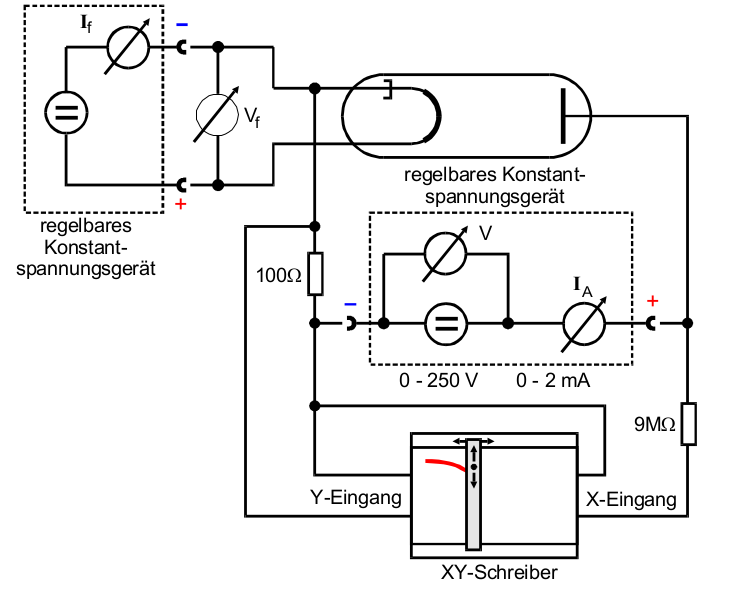
\includegraphics[height=8cm]{SommerAlbum15/Aufbau.png}
  \caption{Versuchsaufbau zur Bestimmung der Kennlinie. Ein XY-Schreiber steht
  in diesem Versuch nicht zur Verfügung.\cite{anleitung}}
  \label{fig:Aufbau}
\end{figure}

\FloatBarrier

Mit Hilfe eines Konstantspannungsgerätes wird ein Heizstrom von
$I_\text{H} = 2-\SI{2.5}{\ampere}$ erzeugt. Die Heizspannung kann an einem
parallel zum Spannungsgerät geschalteten Voltmeter abgelesen werden.
Der erzeugte Anodenstrom wird mit einem in Reihe geschalteten Amperemeter und
einem parallel geschalteten Voltmeter abgelesen.

\begin{figure}
  \centering
  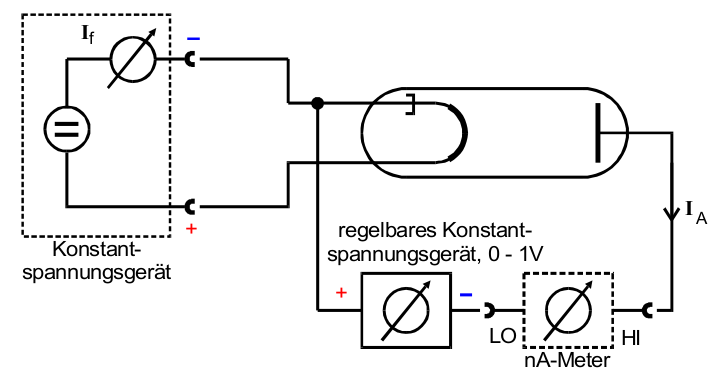
\includegraphics[height=5.5cm]{SommerAlbum15/Aufbau2.png}
  \caption{Versuchsaufbau zur Bestimmung der Anlaufstromkurve.\cite{anleitung}}
  \label{fig:Aufbau2}
\end{figure}

\FloatBarrier

In Abbildung \ref{fig:Aufbau2} ist die Schaltung zur Bestimmung der
Anlaufstromkurve dargestellt. Da die Anlaufströme sehr klein sind, wird ein
empfindliches Amperemeter mit einem möglichst kurzen Kabel an die Anode
geschaltet. Zudem wird ein regelbares Konstantspannungsgerät parallel
zur Diode geschaltet, damit eine geringe Gegenspannung $U = 0-\SI{1}{\volt}$
angelegt werden kann.

\subsection{Messprogramm}

\subsubsection{Aufnahme der Kennlinien}

\begin{enumerate}

\item Zunächst wird der Versuchsaufbau aus Abbildung \ref{fig:Aufbau}, ohne den
XY-Schreiber, aufgebaut.

\item Für fünf verschiedene Heizströme $I_\text{H}$ wird jeweils eine
Kennlinie mit $32$ Spannungs-Werten aufgenommen.

\end{enumerate}

\subsubsection{Aufnahme des Anlaufstromgebiets}

\begin{enumerate}

\item Zunächst wird der Versuchsaufbau aus Abbildung \ref{fig:Aufbau2} aufgebaut
und der maximale Heizstrom von $I_\text{H} = \SI{2.5}{\ampere}$ eingestellt.

\item Für insgesamt $a$ verschiedene

\end{enumerate}
